\chapter{OBDH with ACS}\label{ch:obdh-acs}

The aim of this assignment is to validate the Attitude Control System (ACS)
with the Processor In the Loop (PIL) technique.
PIL consists on simulation from the external environment
through mathematical models (in Simulink)
that are directly connected to the onboard computer.
This way, we can analyze the system's behaviour
based on simulated readings and actuations performed by the OBSW.

The reduced version of an OBSW
is used with the ACS of the UPMSat-2 satellite.
The ACS uses magnetic sensors (magnetometers) and actuators (magnetorquers).
This system conforms to a magnetic attitude control (figure~\ref{fig:acs}).

\begin{figure}[hbtp!]
	\centering{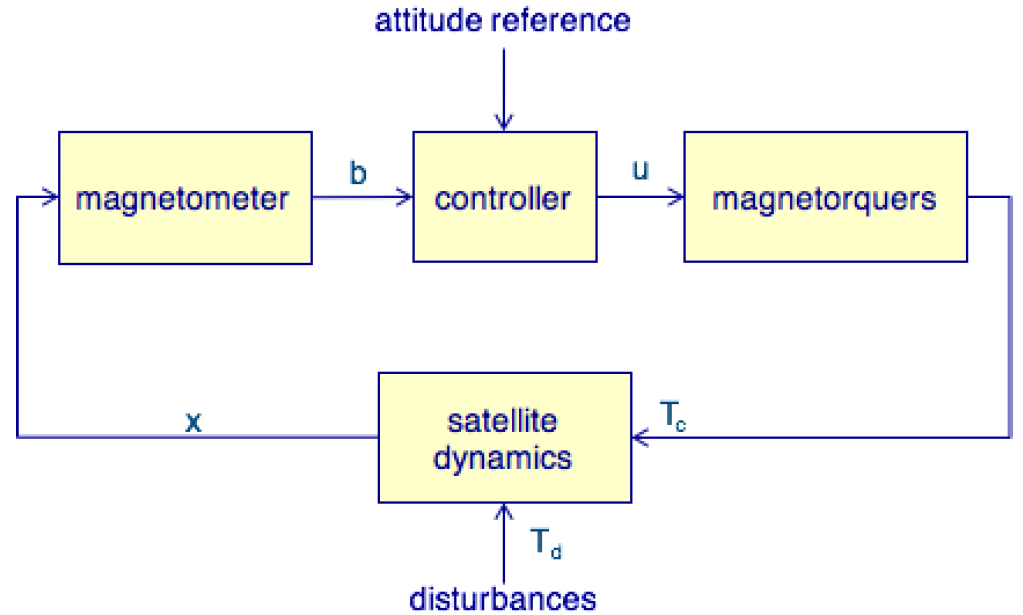
\includegraphics[width=.6\textwidth,keepaspectratio]{acs.png}}
	\caption{Magnetic attitude control system.}
	\label{fig:acs}
\end{figure}

\textbf{Magnetometers} are magnetic sensors
that provide a measurement of the strength
and direction of the magnetic field, i.e. the magnetic field vector,
at a given point.
\textbf{Magnetorquers} are magnetic coil which produce a magnetic moment that interacts with the Earth's field,
thus enabling the attitude of the satellite to be changed.

% -- MIL ------------------------------------------------------------------------

\section{Model In the Loop (MIL) validation}

Software validation usually includes testing the system under real operating conditions.
However, for obvious reasons, on-board space software as well as many other embedded systems cannot be tested in this way.
Simulation models are commonly used in these cases.

The first validation phase uses a model of the ACS,
together with models of the space environment and the spacecraft dynamics,
to assess the validity of the control law and the design parameters (figure~\ref{fig:acs-hl}).
This is usually carried out by a control engineer using a simulation tool.
Simulink is commonly used for ACS development.

\begin{figure}[hbtp!]
    \centering{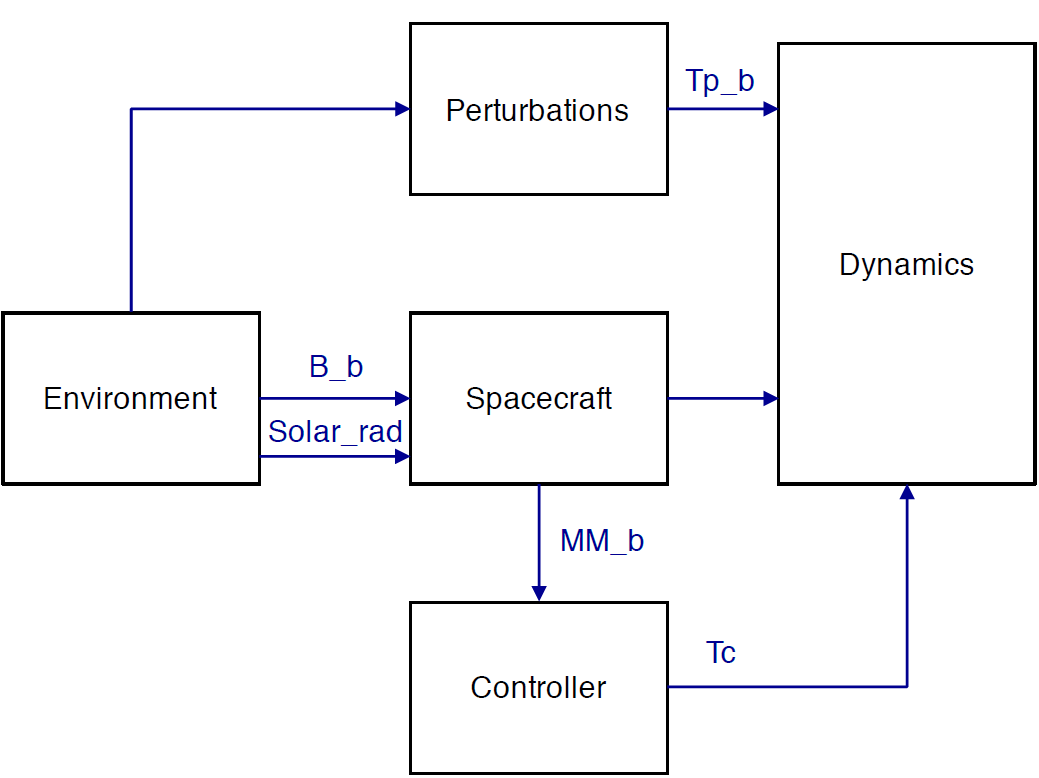
\includegraphics[width=0.6\textwidth,keepaspectratio]{acs-hl.png}}
    \caption{UPMSat-2 ACS high level model view.}
    \label{fig:acs-hl}
\end{figure}

The ACS Simulink model can be simulated by running MATLAB from the
\textcolor{mPurple}{\texttt{lab-4/acs}}
directory and opening \texttt{ACS.slx}.
Three new windows will pop-up: the Simulink window with the ACS model
and two scope windows that show the angular velocity of the satellite in body reference and the actuation over its three magnetorquers.

The Simulink window (figure~\ref{fig:acs-simulink}) shows the high level blocks: the satellite's model is located in the middle (turquoise block),
its dynamics and the models of the Earth's field and Sun with the perturbations.

\begin{figure}[hbtp!]
    \centering{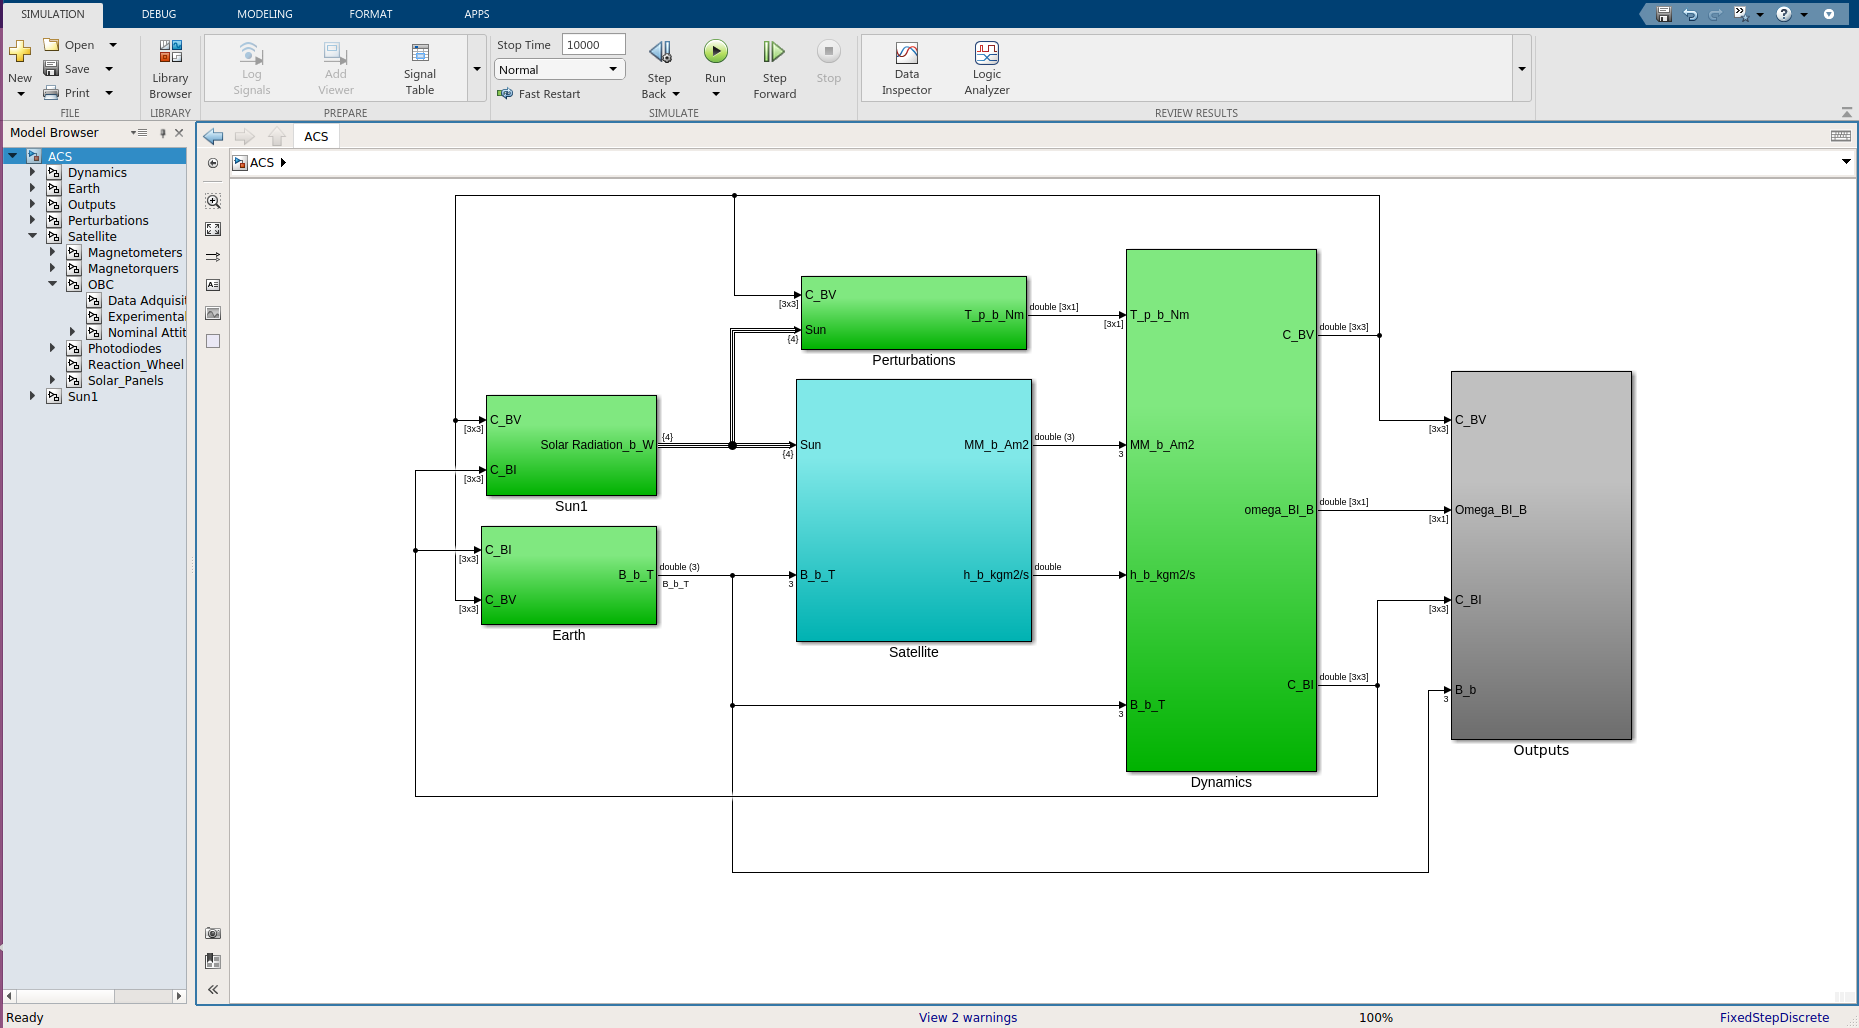
\includegraphics[width=\textwidth,keepaspectratio]{acs-simulink.png}}
    \caption{UPMSat-2 Simulink model.}
    \label{fig:acs-simulink}
\end{figure}

The nominal attitude control can be visualized
by selecting Nominal Attitude Control in the Model Browser menu
(left part of simulink window) or by clicking on Satellite $\rightarrow$ OBC $\rightarrow$ Nominal Attitude Control blocks. The Nominal attitude control has three blocks (figure~\ref{fig:nac}):
\begin{description}
\item[Sensor] samples the analog inputs of the magnetometers. The inputs are converted to engineering units using calibration data.
\item[Control] implements the attitude control law that computes the control action to be output to the magnetorquers.
\item[Actuator] activates the magnetorquers according to the computed control action.
\end{description}

\begin{figure}[H]
            \centering{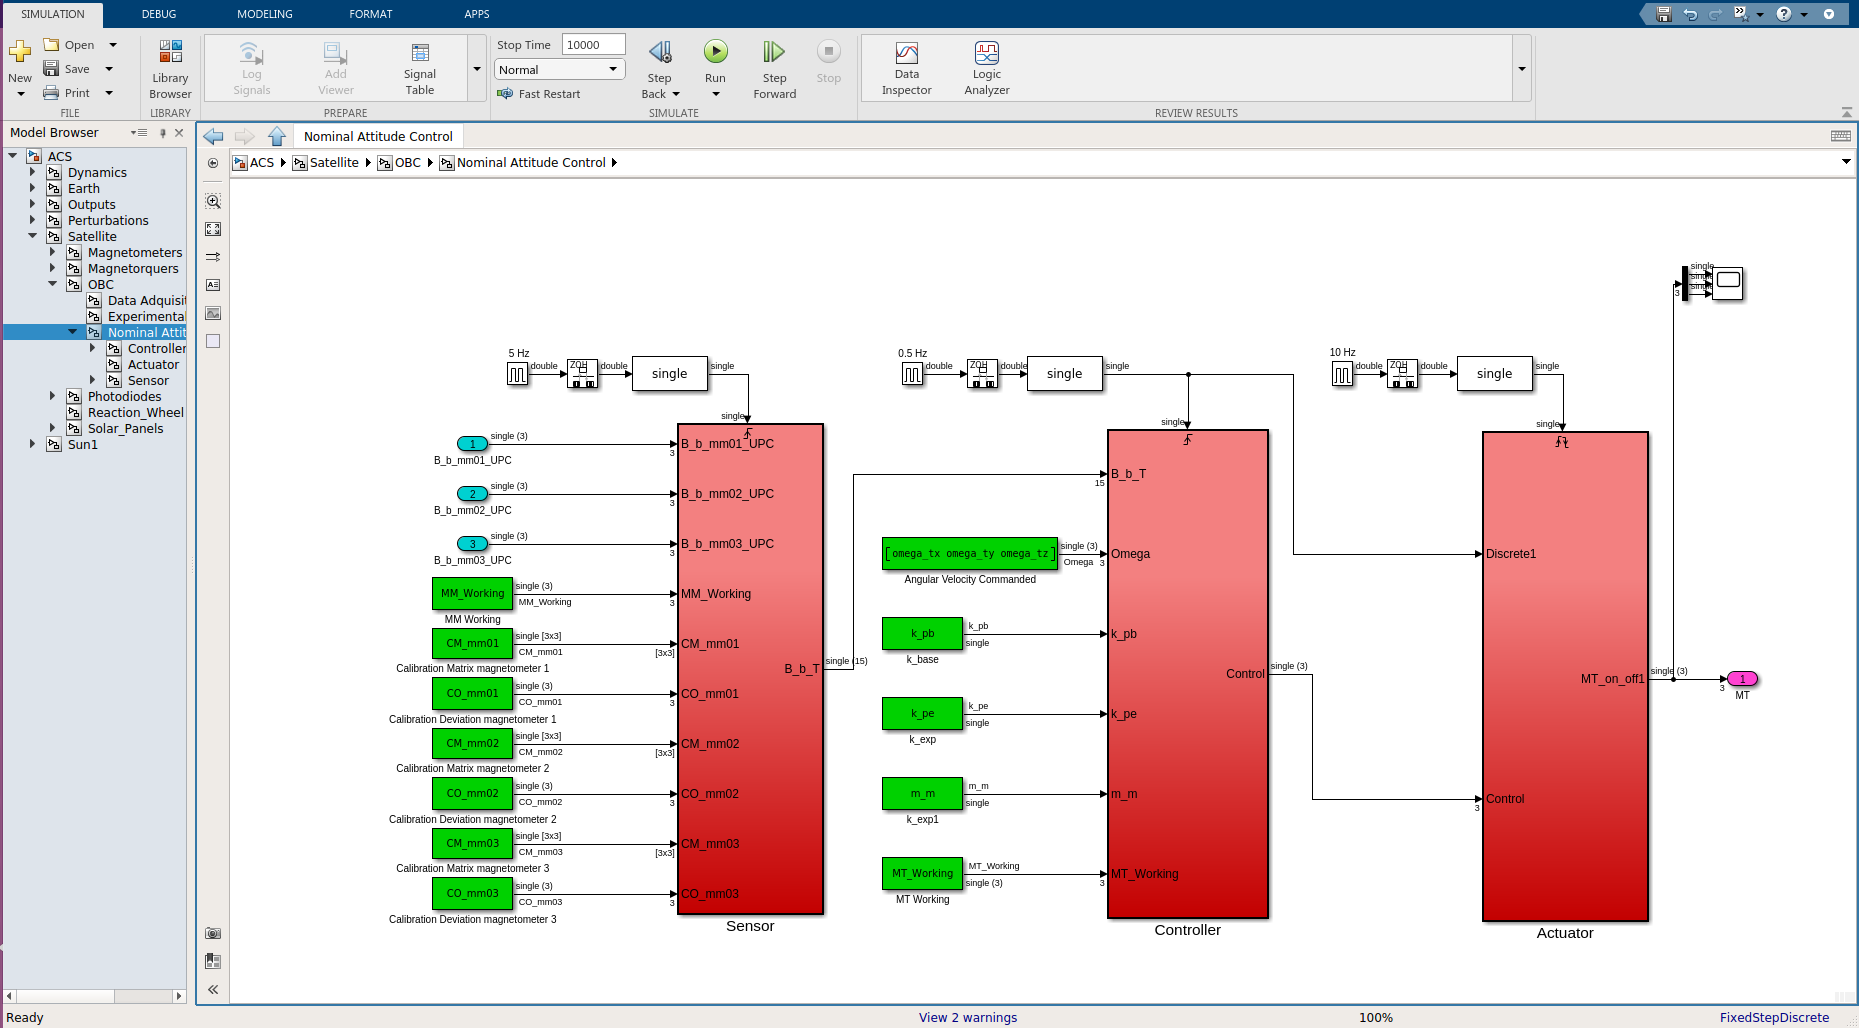
\includegraphics[width=\textwidth,keepaspectratio]{nac.png}}
            \caption{Nominal attitude control.}
            \label{fig:nac}
\end{figure}

To simulate the model an verify its behaviour,
click on Run bottom.
The evolution of the angular velocity of the satellite
and the actuation over the three magnetorquers will be shown in the corresponding scope windows.
The commanded angular velocity set-point is [0, 0, 0.1] rad/s
and the result of the simulation (figure~\ref{fig:scope})
shows the evolution from the initial angular velocity ([0.1, -0.1, -0.1] rad/s).

\begin{figure}[h]
    \centering{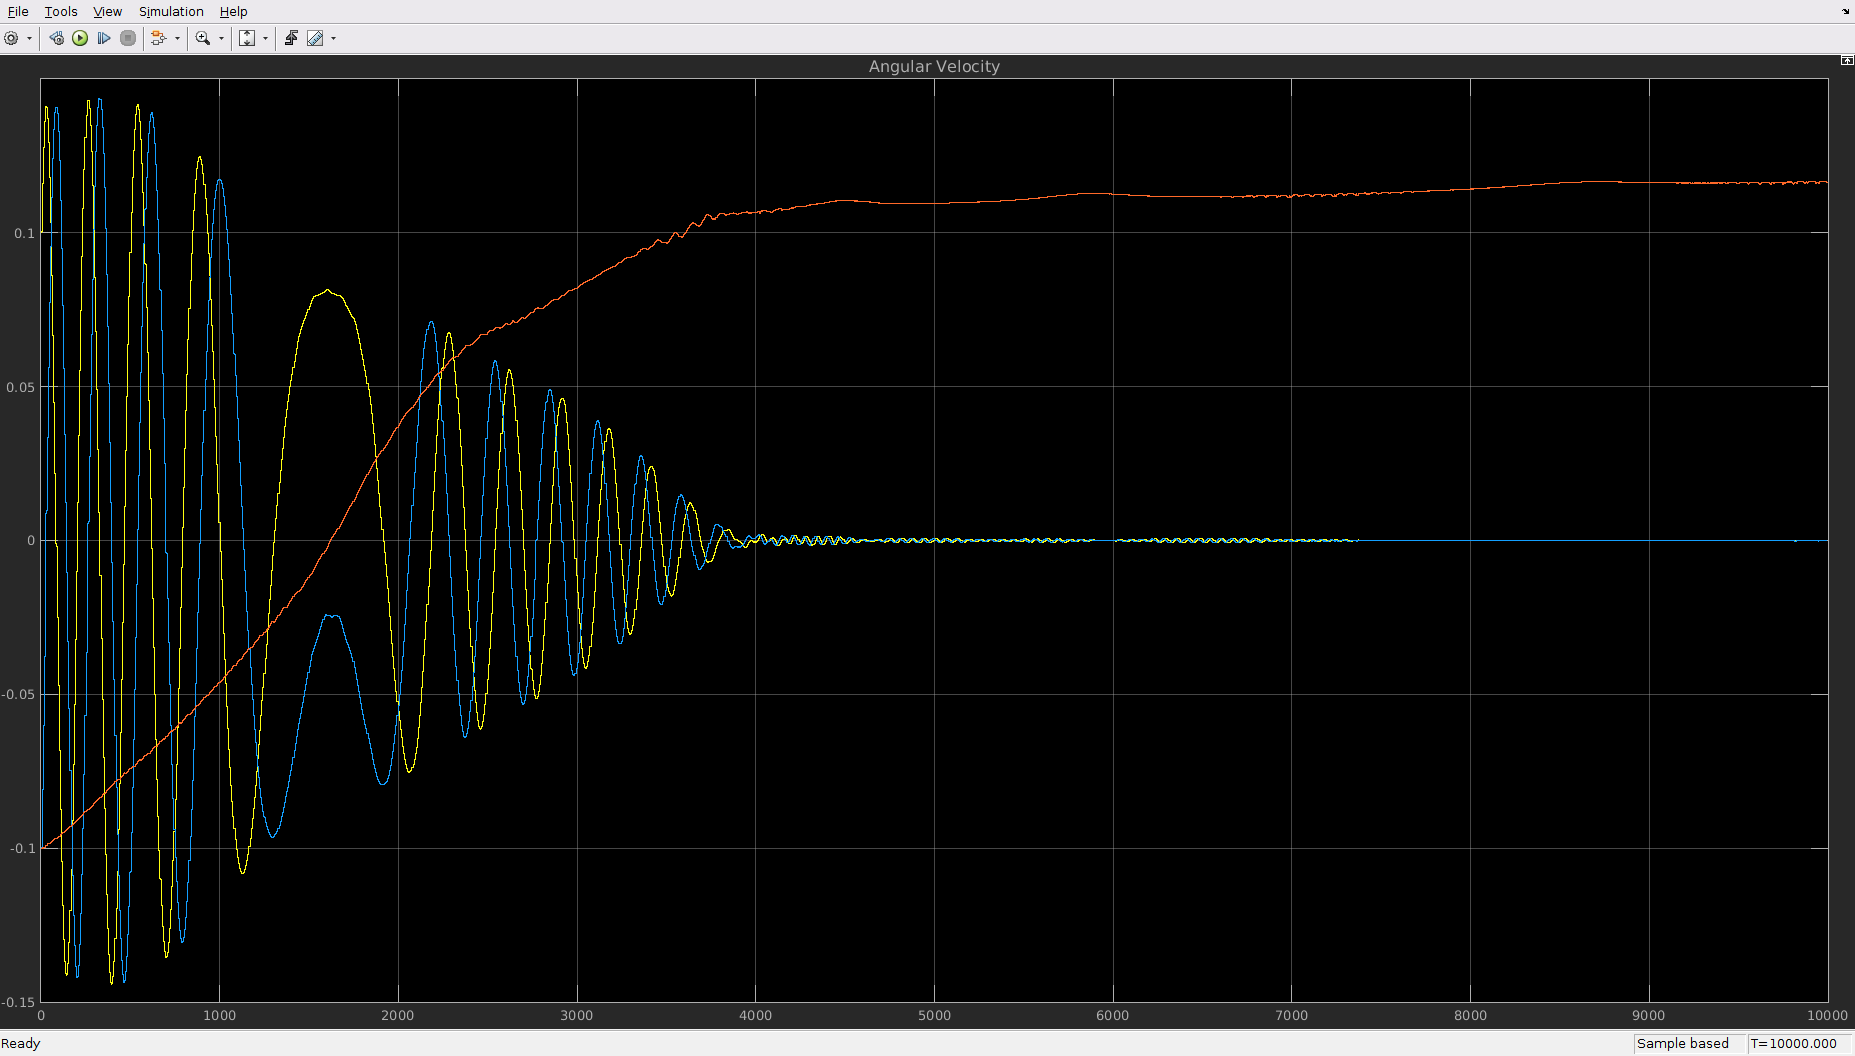
\includegraphics[width=\textwidth,keepaspectratio]{scope.png}}
    \caption{Angular velocity evolution.}
    \label{fig:scope}
\end{figure}

\section{Code generation}

The next step is to execute the ADCS on the board.
In this assignment, only the \texttt{Control} block will be executed on the target board.
The corresponding code can be generated by using the \textbf{Embedded Coder} toolbox but it is needed to isolate \texttt{Control} block from the ACS model.
It can be done by clicking in the Control block,
selecting all the block content (except the trigger block)
and saving it in a new model.

This model named \texttt{control.slx} can be found in \textcolor{mPurple}{\texttt{lab-4/acs}} directory.
Open it with MATLAB and then select APPS in the top menu,
Embedded Coder will appear.
If not, it must be installed by clicking Get Add-Ons and searching it.
The Embedded Coder window (figure~\ref{fig:control}) will appear after clicking on Embedded Coder icon.

\begin{figure}[h]
	\centering{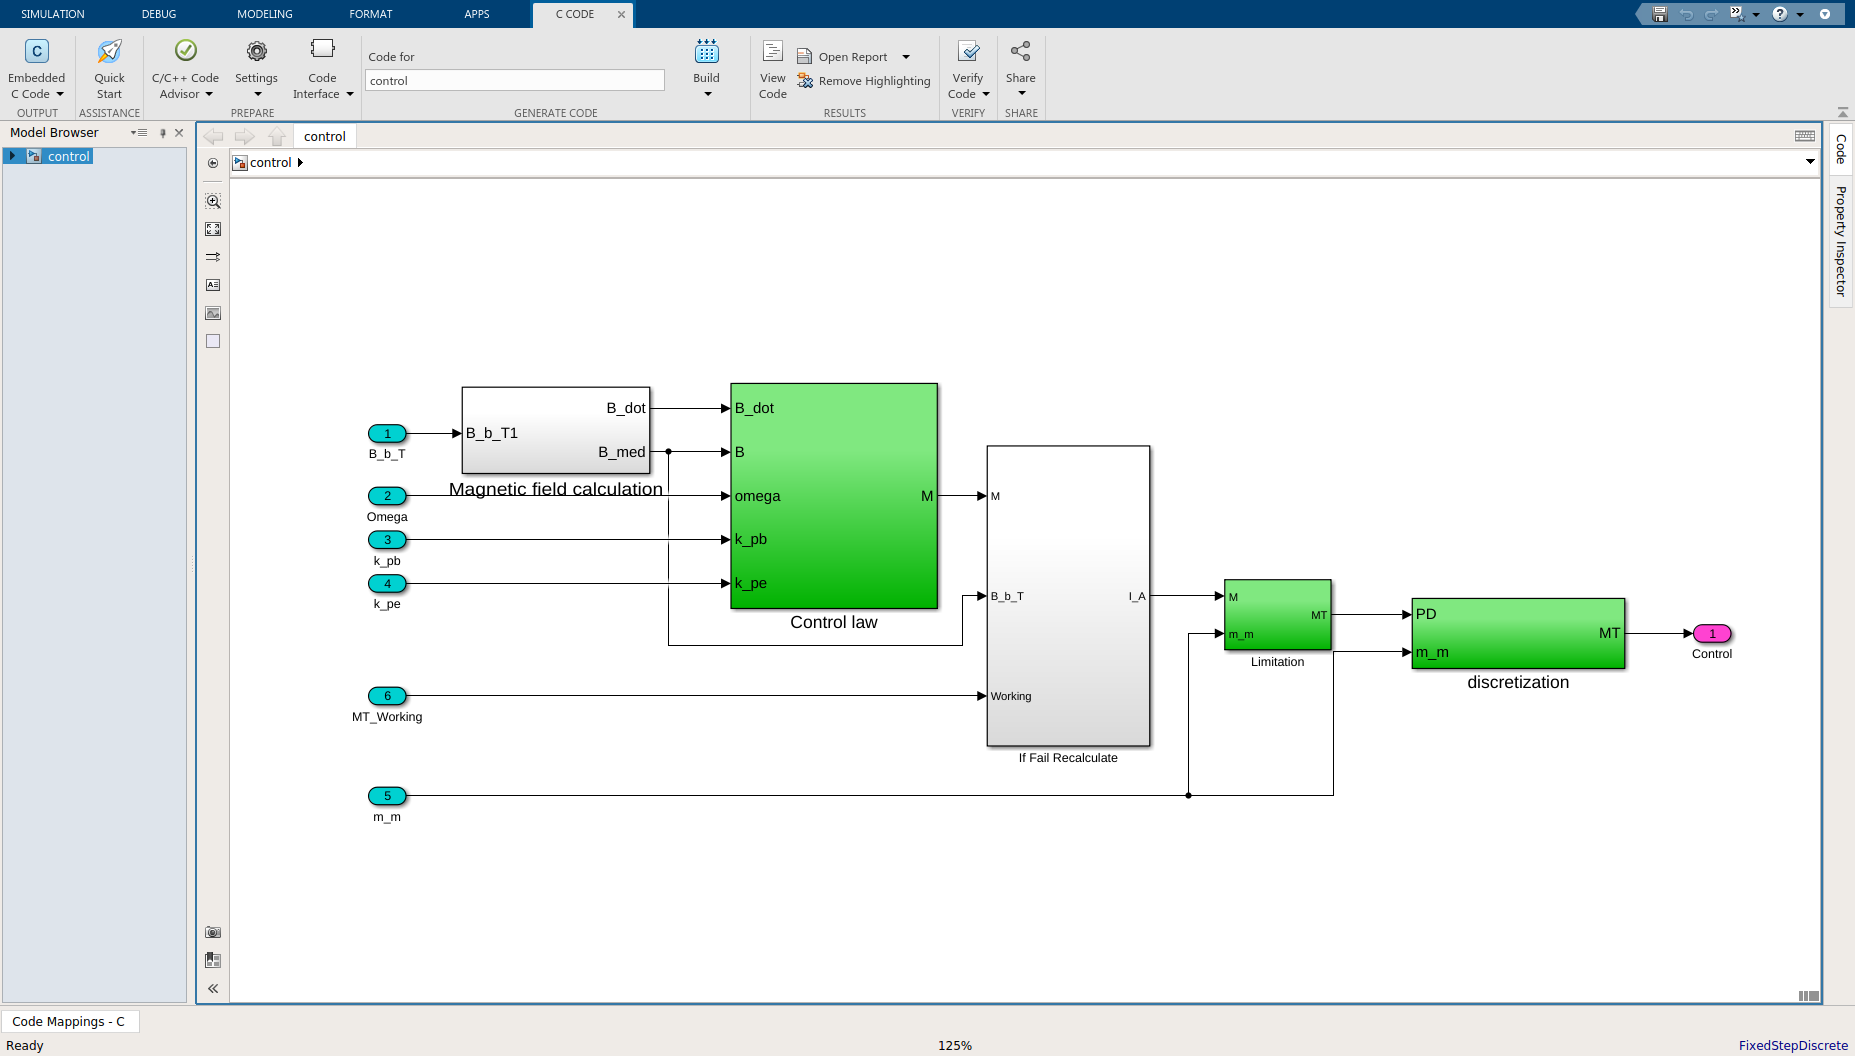
\includegraphics[width=\textwidth,keepaspectratio]{control.png}}
	\caption{Embedded Coder toolbox.}
	\label{fig:control}
\end{figure}

The code generation option as well as characteristics of the target hardware
can be set by clicking on the Settings menu.
The \texttt{control.slx} model has already the proper options,
therefore you can take a look but be carefully and do not modify them.

Now, the code can be generated by clicking on the Build menu.
Once upon the code is generated,
a code generation report window appears.
It is possible to explore the generated code together with different code metrics.
Click on \texttt{control.h} and look for lines 50-79 (figure~\ref{fig:code}) where the generated code interface is located.

\begin{figure}[hbtp!]
    \centering{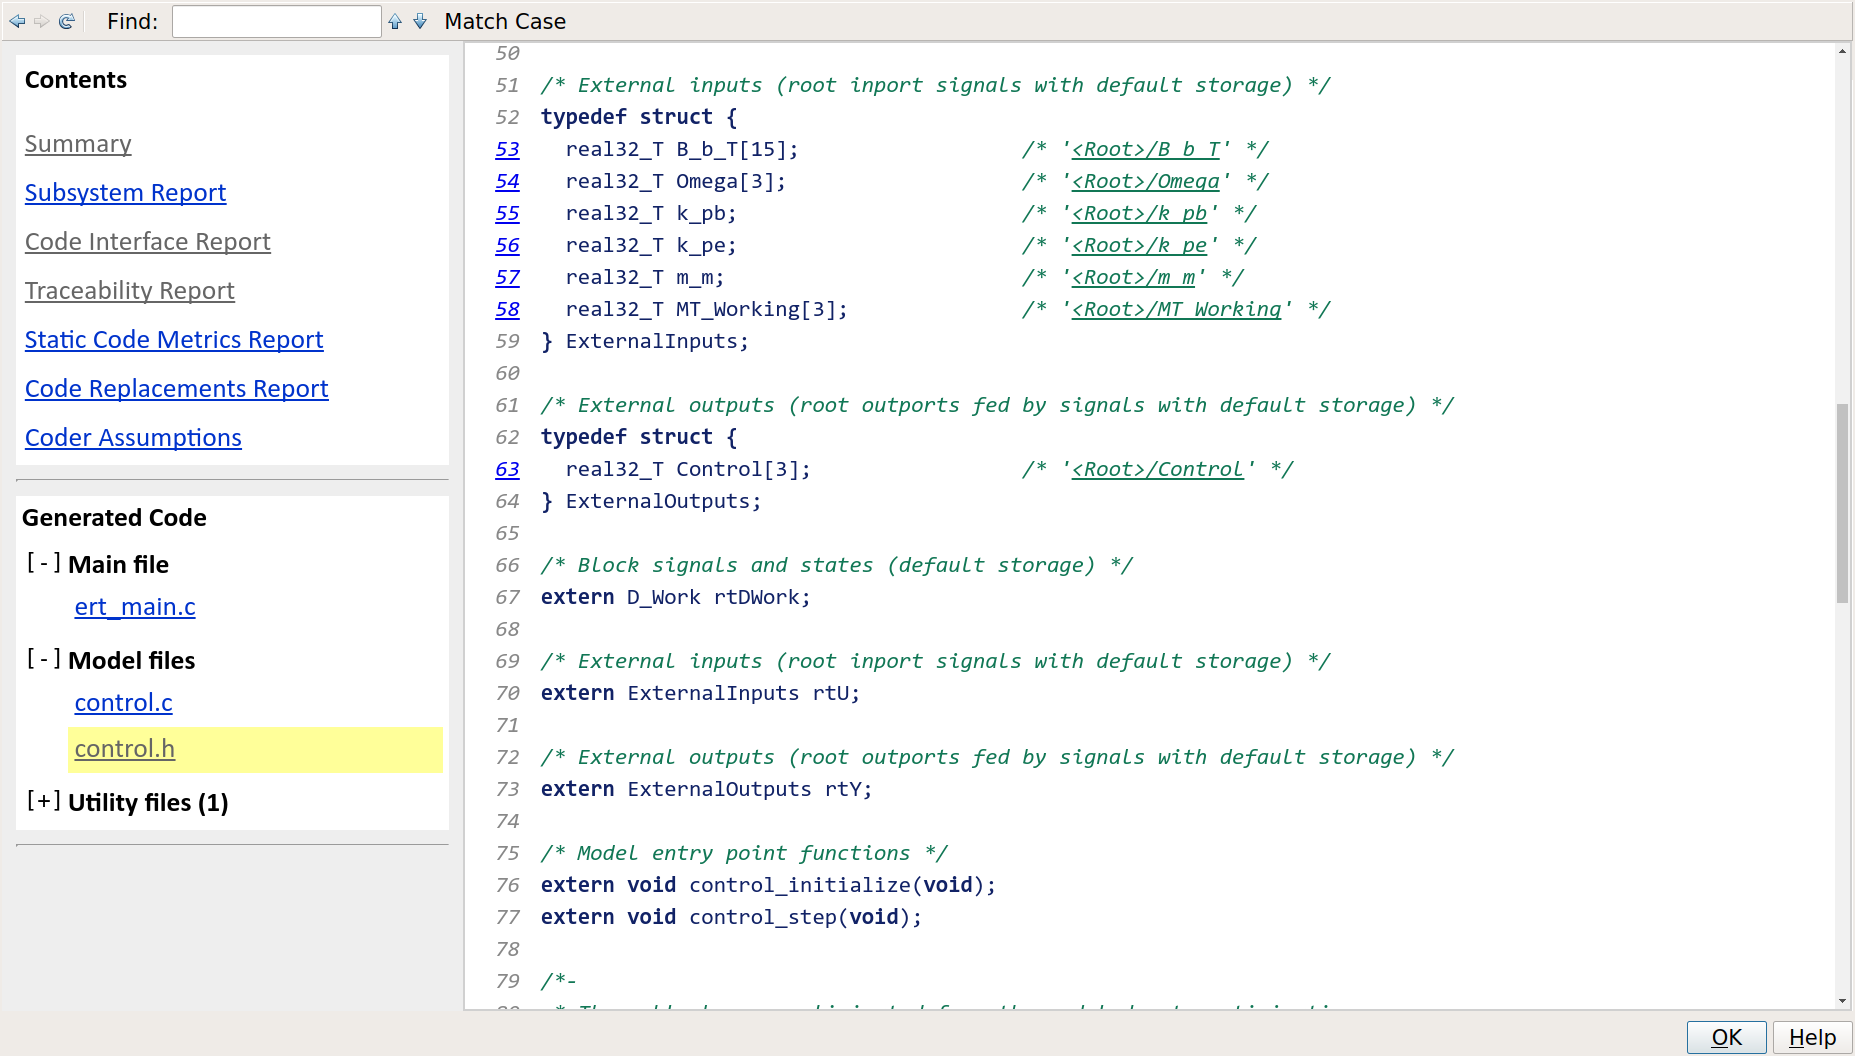
\includegraphics[width=\textwidth,keepaspectratio]{code.png}}
    \caption{Code generation report.}
    \label{fig:code}
\end{figure}

There are two record type definitions (C structs) called \texttt{ExternalInputs} and \texttt{ExternalOutputs}
that are used to interchange data with the blocks
Sensor and Actuator (figure~\ref{fig:nac}).
Data are interchanged with two global variables: \texttt{rtU} and \texttt{rtY}.
Moreover, function \texttt{control\_initialize}
initializes the control code and function \texttt{control\_step}
performs the control algorithm.
The generated code will be embedded in the OBSW by taking into account this interface.

\section{Software architecture}

The implementation code, as initially provided to the students, can be downloaded from \url{https://github.com/STR-UPM/SEU-OBDH-Lab/ass-3}.

\begin{figure}[H]
            \centering{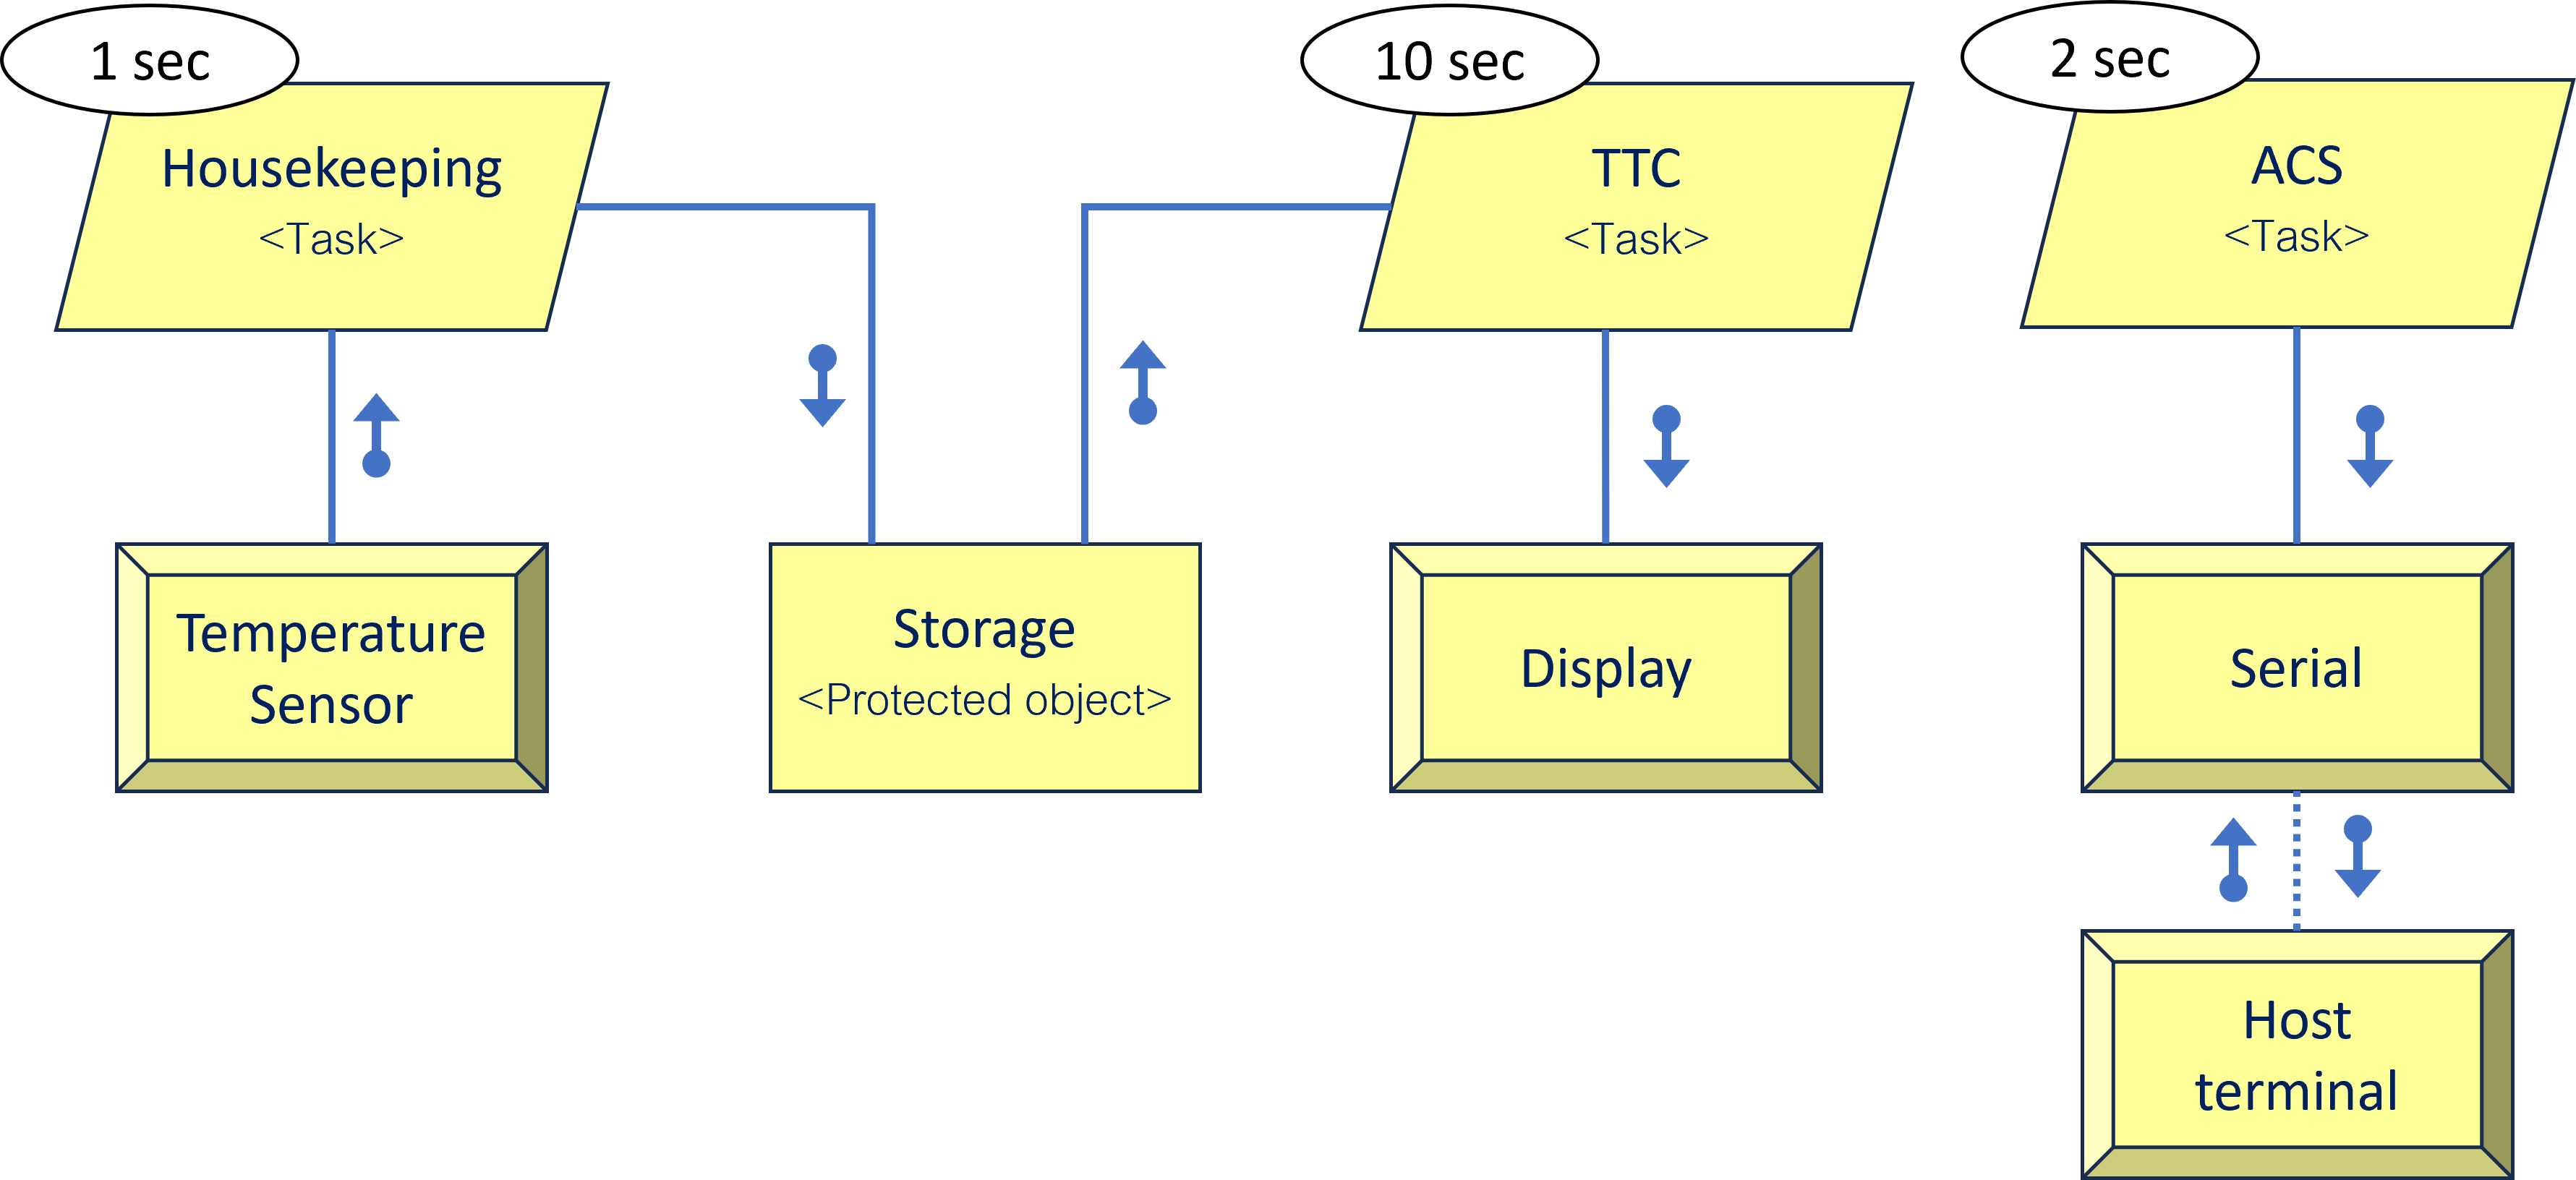
\includegraphics[width=\textwidth,keepaspectratio]{obsw-acs-v2.png}}
            \caption{Software architecture of OBSW with ACS.}
            \label{fig:obdh-acs}
\end{figure}

The software architecture of the OBSW with ACS is depicted in figure~\ref{fig:obdh-acs} and the differences with the previous architecture (figure~\ref{fig:obdh}) are:

The ADCS package is the root element of the ADCS. Its specification consists of one procedure, Initialize, that starts the operation of the component. It has three subpackages:
\begin{description}
\item[ADCS] is the root package of the subsystem and contains a concurrent task, ADCS\_Task that reads the magnetic field vector, calculates the torque vector and sends it to magnetorquers. It also toggles the red LED every two second.
The body of this package uses the generated code by setting the inputs, calling the functions and retrieving the outputs following the interface of figure~\ref{fig:nac}.
\texttt{ADCS\_Task} performs the control algorithm by calling \texttt{control\_step}.
This is shown in figure~\ref{fig:acs-body}.
It uses Export and Import pragmas to interface the generated C code.

\begin{figure}[h]
            \centering{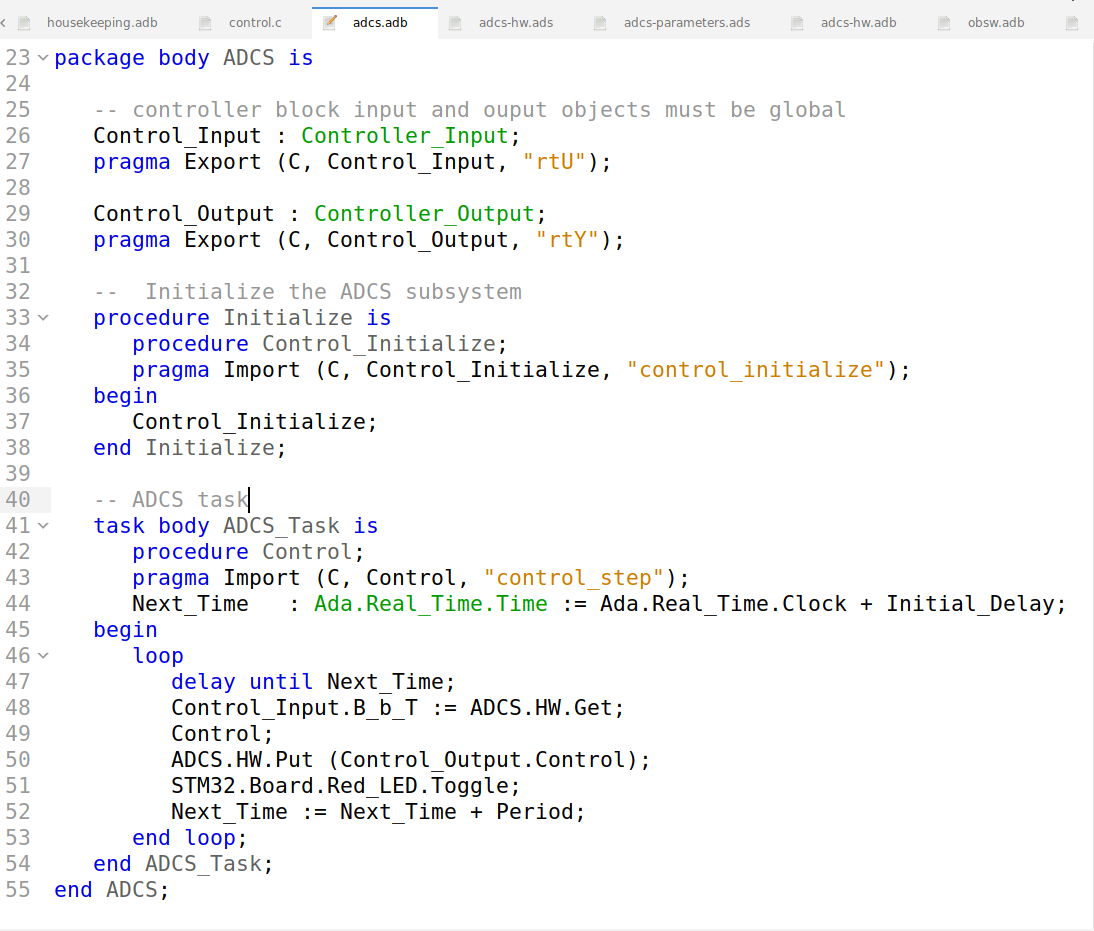
\includegraphics[width=\textwidth,keepaspectratio]{acs-body.png}}
            \caption{Implementation of ACS package.}
            \label{fig:acs-body}
\end{figure}

\item[ADCS.Parameters] contains the definitions of the data types used in the subsystem and parameters that are used to tune the control algorithm. These parameters can be changed by telecommand in the UPMSat-2 OBSW. The data type Controller\_Input is used to read the magnetic field vector in teslas, which are IEEE single precision float numbers. The data type Controller\_Output are used to send the actuation to magnetorquers in newton-meters, which are IEEE single precision float numbers. These data types correspond to the generated C structs ExternalInputs and ExternalOutputs (see figure~\ref{fig:code}), taking advantage of the C and Ada languages interoperability.

\item[ADCS.HW] is in charge of getting the magnetic field vector and putting the
torques. It hides the details of the hardware. Its specification includes the \texttt{Put} and \texttt{Get} subprograms.
This package uses the serial port to interchange magnetic field and torque values with the Software Validation Facility (SVF).
\end{description}

The SVF is an auxiliary computer (the student's PC),
linked to the OBC by a serial line, to run a simulation model of the Earth's magnetic field and satellite dynamics. In this way, engineering values (Nm and T) can be interchanged.

Host computers are also used as SVF by executing a Simulink\texttrademark model of the Earth's magnetic field and satellite dynamics.

In this assignment, the serial line is used to interchange data between ADCS and SVF. Therefore, housekeeping telemetry are send to a text console that is simulated on the host computer, using a mechanism called semihosting. When the target board is connected to the host by means of the ST-LINK USB cable, and the embedded program is run using the debugger in the host, the standard output is re-directed to the debugger console. The GPS environment supports semihosting.

\section{Compile and run with the debugger.}

Open GPS and do the following:
\begin{enumerate}
\item Select Open project on the welcome window. Navigate to the OBSW directory and open the realtime\_housekeeping.gpr project file.
\item Build the executable and load it into the board by clicking on the \hbox{
\includegraphics[width=1.5em]{debug.png}} symbol in the tool bar (or select Build $\rightarrow$ Bareboard $\rightarrow$ Debug on board on the top menu).

The program will be compiled, and the executable will be loaded into the board memory by the debugger. The debugger console (lowest window in GPS) shows the following lines:
\begin{verbatim}
...
(gdb) monitor reset halt
(gdb)
\end{verbatim}

\item Type continue or just c on the debugger console (or select Debug $\rightarrow$ Continue on the top menu).
\begin{verbatim}
(gdb) c
Continuing.
[program running]
\end{verbatim}

After that, the program starts to run on the board and temperature reads are displayed on Messages tab of the debugger window. However, the Red LED does not blink because ACS is waiting sensor inputs from SVF.
\end{enumerate}

% -- PIL ------------------------------------------------------------------------

\section{Processor In the Loop (PIL) validation}

The SVF shall provide sensor inputs and retrieve magnetotorquer outputs. To do that, the remain part of the original simulink model will be used, i.e. all the blocks except the Sensor block.

This model named ACS\_PIL.slx can be found in \textcolor{mPurple}{\texttt{lab-4/acs-pil}} directory. Open it and again three new windows will be pop-up: the Simulink window with the \texttt{ACS\_PIL} model
and two scope windows that show the angular velocity of the satellite in body reference and the actuation over the three magnetorquers.

The \texttt{Control} block of this model has been substituted by serial link connections as shown in figure~\ref{fig:nac-pil}. Identify the serial port name on the host computer and edit the serial configuration block by selecting the serial line of your PC.

\begin{figure}[h]
            \centering{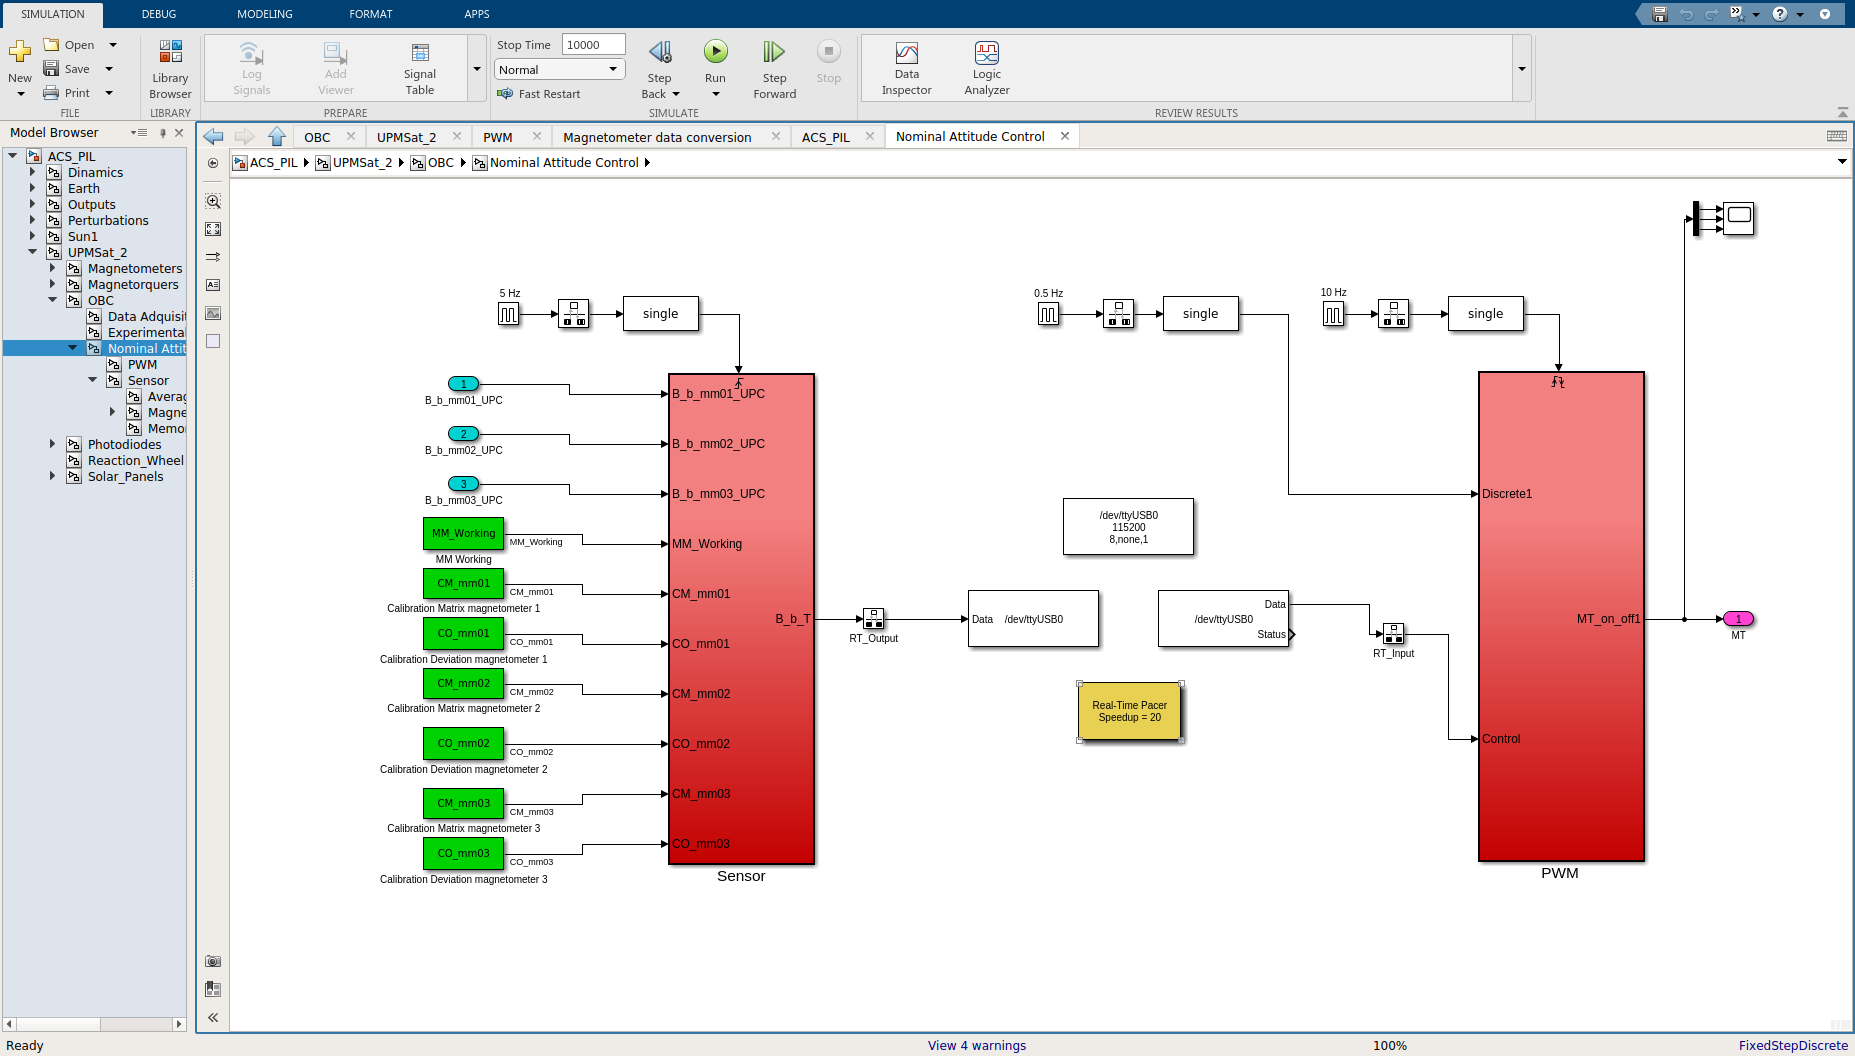
\includegraphics[width=\textwidth,keepaspectratio]{nac-pil.png}}
            \caption{Nominal attitude control for PIL.}
            \label{fig:nac-pil}
\end{figure}

Additional rate transition blocks has been added for a proper communication and a Real-Time Pacer block has been also added to set the simulation speed. In a real case, an speedup equal to 1 should be used but it is to slow.

Start the simulation and verify angular velocity stabilization. Now ADC runs and red LED is toggled. 

\section{Make changes to the simulation}

\begin{itemize}
\item Default parameters for control blocks can be changed in Ada source file ACS-parameters.ads.
\begin{itemize}
\item \texttt{Default\_omega} is the consigned angular velocity.
\item \texttt{Default\_MT\_Working} contains the operational magneto-torques.
\end{itemize}

In UPMSat-2 many parameters can be changed by TC.
\item The initial angular velocity can be changed in Simulink source file initialization.m.
\begin{itemize}
\item omega\_BI\_B0 = [0.1;-0.1;-0.1];
\end{itemize}
\end{itemize}
